\documentclass{article}
\author{Giuliano Abruzzo}
\title{Software Engineering Notes}
\usepackage{geometry}
\usepackage{float}
\usepackage{graphicx,array}
\usepackage{algorithm}
\usepackage[noend]{algpseudocode}
\usepackage{caption}
\newcolumntype{C}[1]{>{\centering\let\newline\\\arraybackslash\hspace{0pt}}m{#1}}
\newcolumntype{L}[1]{>{\raggedright\let\newline\\\arraybackslash\hspace{0pt}}m{#1}}
\input{insbox}
\DeclareCaptionFormat{myformat}{#3}
\captionsetup[algorithm]{format=myformat}

\begin{document}

\maketitle
\newpage
\tableofcontents
\newpage
\section{Cap 1: Software Process Standardization}
A \textbf{process model} is a \emph{structured collection of practices} that describe the characteristics of effective \emph{processes}. A \emph{process model} is used:
\begin{itemize}
\item To set process \emph{measurable objectives} and \emph{priorities};
\item To ensure \emph{stable, capable}, and \emph{mature processes};
\item As a \emph{guide} for improvement of \emph{projects} and \emph{organizational processes};
\item To diagnose/certify the \emph{state} of an \emph{organization's current practices};
\end{itemize}
\textbf{Capability Maturity Model Integration} or \textbf{CMMI} is a \emph{process improvement approach} that provides organizations with the \emph{essential elements} of \emph{effective processes}. It is a \emph{constellation} of components which generate \emph{process model} called \textbf{CMMI best practices}. These \emph{constellations} are:
\begin{itemize}
\item \textbf{CMMI-DEV}: which provides guidance for \emph{managing, measuring} and \emph{monitoring development processes};  
\item \textbf{CMMI-SVC}: which provides guidance for \emph{delivering services} within organizations and to external customers;
\item \textbf{CMMI-ACQ}: which provides guidance for \emph{applying CMMI best practices} in an acquiring organization;
\end{itemize} 
There are several \textbf{capability levels} of a \emph{process}, and they can be described as a \emph{pyramid}:
\begin{figure}[H]
  \centering
  \includegraphics[scale=1.1]{cattura.png}
\end{figure}
\hfill \break
\textbf{Process management}, \textbf{Project management}, \textbf{Engineering} and \textbf{Support} are the 4 groups of \emph{process areas} related to \textbf{CMMI framework}. \\\\\textbf{ISO 12207} \emph{standard} for \emph{software lifecycle processes} defines and structures all \emph{activities} involved in the \textbf{Software Development Process}. Is based on two principles: 
\begin{itemize}
\item \textbf{Modularity}: \emph{processes} with \emph{minimum coupling} and \emph{maximum cohesion};
\item \textbf{Responsibility}: establish \emph{responsibility} for each \emph{process};
\end{itemize}
\pagebreak
\textbf{ISO 9000} \emph{standard} addresses \emph{quality management}, used by any organization which \emph{design, develops, manages} any \emph{product} or provi\emph{}des any form of \emph{service}, it achieves customer satisfaction and continual improvement. The \emph{ISO 9000} fundamental \textbf{building blocks} are:
\begin{itemize}
\item \textbf{Quality management system};
\item \textbf{Management responsibility};
\item \textbf{Resource management};
\item \textbf{Product/Service realization};
\item \textbf{Measurement, analysis, and improvement};
\end{itemize}
\section{Cap 2: Software Processes}
Since \emph{software products} are not \emph{tangible}, we have to use \textbf{special methods} in order to manage them, especially during their \emph{development}. The \emph{monitoring} is based on the explicit definition of \emph{activities} to be performed and \textbf{documents} to be produced. \emph{Documents} allows to \emph{monitor} the \emph{evolution} of the \emph{process} so we can evaluate its \emph{quality}. There are several \textbf{software process models}:
\begin{itemize}
\item \textbf{Waterfall model}: 
\begin{itemize}
\item It provides several stages: \emph{analysis, design, implementation and unit test, integration and system test, maintenance}. This can be a \textbf{problem}, cause discovering \emph{errors} at the \emph{end} is not good, the \emph{end user} has not a clear idea about the \emph{project} until it's finished, and \emph{changes} are difficult to apply after the \emph{process} is started;
\end{itemize}
\item \textbf{Prototypal model}:
\begin{itemize}
\item In which the \emph{customer interaction} is \emph{contiguous} and we present to it every time the \emph{prototype}. The goal is to collect and disambiguate requirement involving the \emph{customer}. The \emph{prototype} are not full working, but since we work with the \emph{customer}, he has an idea about the \emph{project}; 
\end{itemize}
\item \textbf{Incremental model}:
\begin{itemize}
\item Similar to the previous one but all the \emph{intermediate version} of the \emph{product} are fully working ones, so it allows a more accurate design.
\end{itemize} 
\end{itemize}
These two \emph{models} were part of the \textbf{incremental development}, where for each versions a part of the required functionality is delivered. With these approach, \emph{system failures} are less probable and the \emph{customer} soon has an idea about the \emph{project} and it is also good for \emph{changes}, obviously;
\begin{itemize}
\item \textbf{Formal models}:
\begin{itemize}
\item They comprise every \emph{method} where there are \emph{formalism} for all step of the process. They are highly precise, but difficult to understand by a human being;
\end{itemize}
\pagebreak
\item \textbf{Spiral model}:
\begin{itemize}
\item There is no sequence for \emph{activities} to be done, but all is represented as a \emph{spiral} where each loop is a \emph{phase}. There are no fixed \emph{stages} like in previous \emph{models}, every \emph{loop} is defined depending on what is required. We have different \emph{sectors} like: \emph{objective setting, risk assessment and reduction, development and validation, planning; }
\end{itemize}
\end{itemize}
The main involved \textbf{activities} in \emph{software processes} are:
\begin{itemize}
\item \textbf{Software specification}: the \emph{process} of establishing what \emph{services} are required, and the \emph{project's constructs}. It's a requirement engineering process;
\item \textbf{Software design and implementation}: the \emph{process} of converting the \emph{system specification} to an \emph{executable system};
\item \textbf{Software validation}: the \emph{process} in which is intended to show that the \emph{system} conforms to its \emph{specification} and meet \emph{customer requirements}, \emph{system testing} belongs to this \emph{activity};
\item \textbf{Software evaluation}: the \emph{process} in which new \emph{features} and \emph{changes} are implemented;
\end{itemize}
\section{SCRUM}
\textbf{Scrum} is an \emph{agile process} that allows us to focus on delivering the highest \emph{business values} in the shortest time. The \emph{business} sets the priorities and teams self-organize to determine the best way to deliver high priority \emph{features}. \emph{Inspections} is done every two weeks (to one month) so anyone can see \emph{real working software} and decide to release it as is or continue to develop it. The procedure is divided in \textbf{sprints} of \emph{software development} (2-4 weeks). \emph{Requirements} of the \emph{project} are captured in a \textbf{product backlog}. 
\begin{figure}[H]
  \centering
  \includegraphics[scale=0.35]{cattura1.png}
\end{figure}
\hfill \break
This sequence is repeated in each \textbf{sprint}, and no \emph{changes} are made during a \emph{sprint}, so there are no problems in \emph{development process}. \emph{Sprint} duration depends in how much time is needed to complete a \emph{feature}, indeed for every \emph{sprint} there is a potentially \emph{shippable product} increment. \\
\clearpage
The \textbf{SCRUM framework} is composed by:
\begin{itemize}
\item \textbf{Roles}:
\begin{itemize}
\item \textbf{Product Owner}: defines \emph{product features}, decide the \emph{release date} and content and rejects/accept the work result;
\item \textbf{Scrum Master}: represent \emph{management} to the \emph{project}, ensures that the \emph{team} is fully functional and productive, enable close cooperation across all roles and functions and shields the \emph{team} from \emph{external interference};
\item \textbf{Team}: typically composed by 5-9 people, it is \emph{cross-functional} and \emph{members} should be full-time. Membership should change only between \emph{sprints};
\end{itemize}
\item \textbf{Ceremonies}:
\begin{itemize}
\item \textbf{Sprint planning}: the phase where \emph{team} selects items from the \emph{product backlog} to commit completing, so \emph{sprint backlog} is created, giving an estimated time for each \emph{task} and this is done collaboratively;
\item \textbf{Daily Scrum}: where the \emph{team} talks about things to do and so on;
\item \textbf{Sprint review}: the team presents what it accomplished during the \emph{sprint};
\item \textbf{Sprint retrospective}: the \emph{team} take a look at what is and is not working;
\end{itemize}
\item \textbf{Artifacts}:
\begin{itemize}
\item \textbf{Product Backlog}: contains \emph{requirement} and a list of all desired work on the \emph{project}. It's ideally expressed such that each \emph{item} has value to the \emph{users} or \emph{customers} of the \emph{product};
\item \textbf{Sprint Backlog}: is isolated to a single \emph{sprint} and contains \emph{goals} for it. It can be manipulated by every \emph{member} of the \emph{team};
\end{itemize}
\end{itemize}
\section{User Stories}
\textbf{User stories} are sentence in everyday language which represent \emph{backlog items}. They fit on 3'' x 5'' \emph{index card} and have a fixed \emph{structure} like: \[\textbf{As a} \emph{ USER},\textbf{ So that } \emph{I CAN ACHIEVE GOAL}, \textbf{ I want to}\emph{ DO SOME TASK}.\]
They can be formulated as \emph{acceptance test} before code is written. As they are \emph{product backlog items}, they have a \textbf{priority}. \emph{User stories} can have an \textbf{achievement score} (\emph{points} in integer scale) depending on their \emph{complexity}, and this allows to check \emph{productivity} calculating number of \emph{points/week}. \emph{Trackers} allows attaching \emph{documents} to \emph{User stories}. In order to understand if we have a good \emph{user story} we use the \emph{SMART stories system}, which stands for \textbf{S}pecific, \textbf{M}easurable, \textbf{A}chievable, \textbf{R}elevant, \textbf{T}imeboxed. Sometimes \emph{User stories} need \textbf{UI}, so in this case we need to attach a \emph{document} to the story: pen and paper drawings or \textbf{Lo-Fi UI}. \textbf{Storyboard} show how \emph{UI changes} are based on \emph{user actions}. 
\clearpage
\section{Distributed Programming}
We can have different types of \textbf{tier architecture}:\\\\
\textbf{1-Tier Architecture}:\\
\begin{tabular}{C{3cm}  L{11cm}}
\includegraphics[scale=0.25]{cattura2.png} &  \newline 
\textbf{Client} is any \emph{user} or \emph{program} that wants to perform an \emph{operation} over the \emph{system}, interacting with the \textbf{presentation layer}. The \textbf{application layer} represents whats the \emph{system} actually does and it can have several forms: \emph{programs, constraints, business processes}. The \textbf{resource manager layer} is the \emph{storage} of the \emph{data} necessary for the \emph{information system} to work. In this design all is centralized and \emph{managing} and \emph{controlling resources} is easier. \\
\end{tabular}\\\\
\textbf{2-Tier Architecture}:\\
\begin{tabular}{C{4cm}  L{10cm}}
        \includegraphics[scale=0.25]{cattura3.png} &  \newline 
        \textbf{Client} are divided and there is the concept of API at a client level, so there are no client connections/sessions to maintain, as the resource manager interacts with application layer only. \\
\end{tabular}\\\\
\textbf{3-Tier Architecture}:\\
\begin{tabular}{C{4cm}  L{10cm}}
        \includegraphics[scale=0.25]{cattura4.png} &  \newline 
        \textbf{Middleware} is just a level of \emph{indirection} between \emph{clients} and other \emph{layers} of the system. It introduces an additional layer of \emph{business logic} encompassing all underlying systems. The \textbf{N-tier architecture} is just a generalization of this schema. \\
\end{tabular}\\\\
In \emph{Middleware} there is extensive use of \textbf{communications}. We know that there are two types of \emph{communication}, \emph{asynchronous} and \emph{synchronous}. \emph{Synchronous} communication requires both the parties to be online, with connection overhead and difficulty to recover from \emph{failures}, in fact \emph{failures} are often handled through \emph{timeouts} and similar technique. To solve this there are two technique:
\begin{itemize}
\item \textbf{Enhanced Support}: \emph{service replication} and\emph{ load balancing} are used in order to prevent the service to be unavailable; 
\item \textbf{Asynchronous Interaction}: with the use of technologies like \emph{non-blocking invocation} or \emph{persistent queues};
\end{itemize} 
As \textbf{Middleware} is a \emph{technique} to hide some complex mechanisms of \emph{information system}, \emph{programming abstraction} can be considered an example. As the \emph{programming abstraction} reach higher and higher levels, the \emph{underlying infrastructure} has to grow accordingly, and it is also intended to support \emph{additional functionality} that makes \emph{development, maintenance} and \emph{monitoring} easier and less costly. \\\\
\textbf{Remote Procedure Calls} or \textbf{RPC} is a \emph{point-to-point protocol} that supports the interaction between two \emph{entities}. \textbf{RPC calls} are treated as independent ones even if the are more \emph{entries} interacting each other. The programmer uses an \textbf{RPC system} instead of implementing a different one for each \emph{distributed system}. An \emph{RPC system} hides low-level operations, provides an interface definition language to describe the services, and generates all the code necessary to made the RPCs work. \textbf{Publish/Subscribe} is a type of \emph{many-to-many communication} where the participants are divided in two groups, \emph{publisher} and \emph{subscriber} and the \emph{communication} takes place through a \emph{central entry}, that is often a \emph{queue} and \emph{infos} can be \emph{topic-based} or \emph{content-based.} The notification to a \emph{subscriber} can be done in two ways: \textbf{push} where \emph{subscribers} are invoked in callback, or \textbf{pull} where \emph{subscribers} poll the central entry when they need messages.
\\\\
This is an example of \textbf{message-oriented Middleware} on internet, where \emph{proxy} and \emph{firewalls} are a way to have \emph{Middleware} on the internet and they work as in this schema:
\begin{figure}[H]
  \centering
  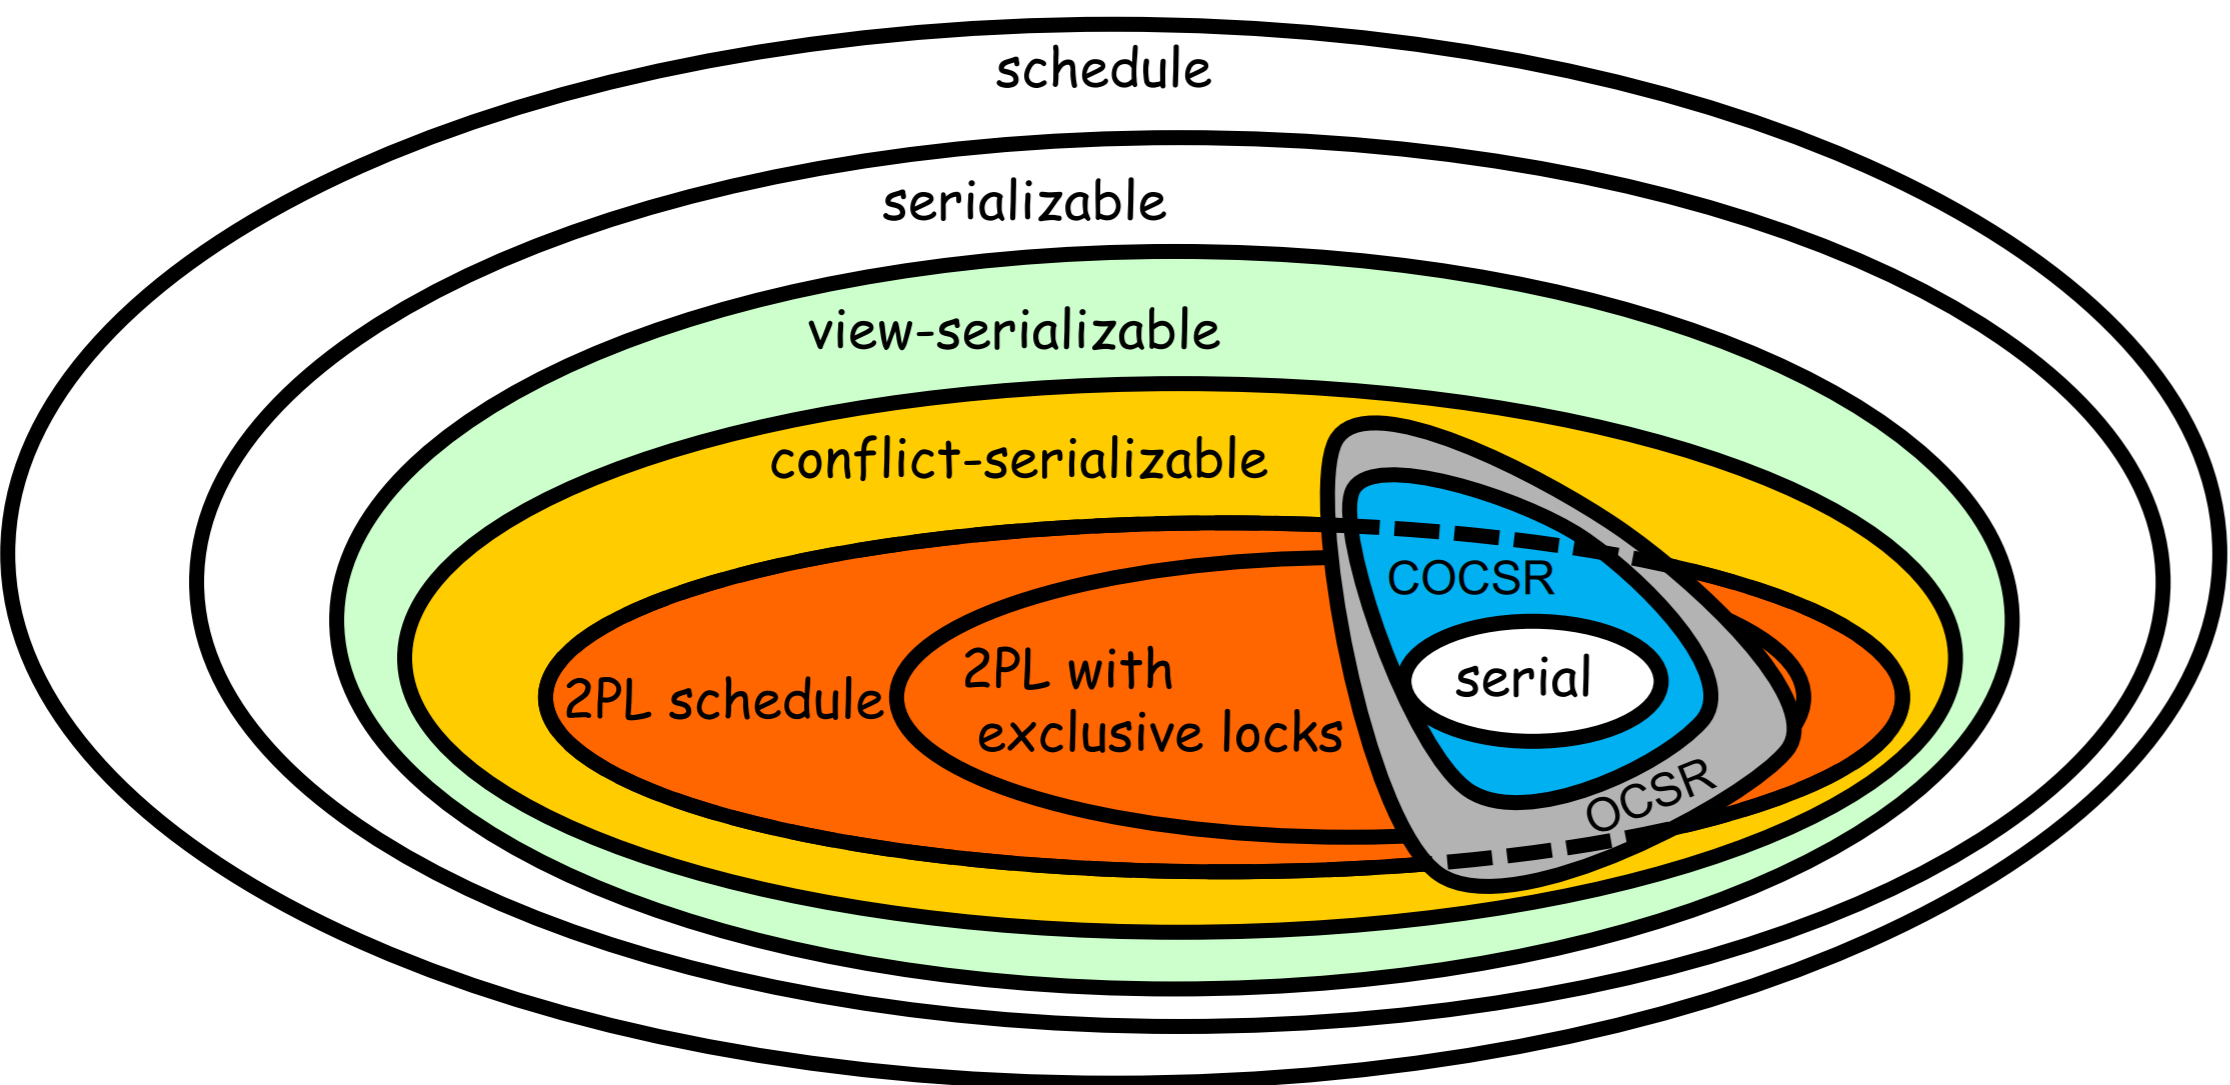
\includegraphics[scale=0.45]{cattura5.png}
\end{figure}
\section{Web Services}
A \textbf{Web Service} is a \emph{programmatically available application logic} exposed over the \emph{internet}, such that \emph{clients} can access \emph{network-available services} instead of invoking available \emph{applications} to accomplish some \emph{task}. \textbf{Web services} perform \emph{encapsulated business functions} such as:
\begin{itemize}
\item A \emph{self-contained business task};
\item A \emph{full-fledged business process};
\item An \emph{application};
\item A \emph{service-enabled resource};
\end{itemize}
\textbf{Services} offered can change depending on \emph{pricing}, in fact there is also a \emph{billing model} which can be different, depending on the \emph{service type} offered \emph{services} can mixed/merged to create \emph{extensions} and so on. This \emph{application logic} appeared at the beginning with \textbf{ASP} or \textbf{Application Service Providers}, an \emph{ASP} "rents" applications to subscribers. The \textbf{ASP} model introduced the concept of \textbf{software-as-service} but suffered from several limitations like inability to \emph{integrate, customize} and \emph{develop} \emph{highly interactive} applications, instead the new architecture of \emph{web services} makes \emph{communications} and \emph{access} to \emph{applications} on the internet easier. \emph{Services} can be used within an enterprise to accomplish some \emph{tasks}, but also between enterprises. \textbf{Services} can mainly be of two types:
\begin{itemize}
\item \textbf{Informational services}: which provide \emph{access} to \emph{content} interacting with an \emph{end-user} by \emph{request/response sequences};
\item \textbf{Complex services}: which invoke the assembly and invocation of many \emph{pre-existing services} in a unique result;
\end{itemize}
\emph{Services} can be \textbf{functional} or \textbf{non-functional}, \emph{functional} if the \emph{service} describe his \emph{overall behavior}, \emph{non-functional} if it describe only some \emph{targets service quality attributes}. \emph{Services} can be \textbf{stateless} and \textbf{stateful}, \emph{stateless} if they can be invoked repeatedly without maintaining a \emph{state} or a \emph{context}, \emph{stateful} if they require their \emph{context} to be preserved from one invocation to the next. \\\\
The \textbf{service model} allows for a clear distinction to be made between:
\begin{itemize}
\item \textbf{Service providers}: who provides the \emph{service};
\item \textbf{Service clients}: who uses the \emph{service};
\item \textbf{Service registry}: the \emph{directory} where \emph{service descriptions} are published and searched;
\end{itemize}
\textbf{SOAP} is the \emph{standard messaging protocol} used by \emph{web services}. \emph{SOAP's application} is \emph{inter application communication} through \emph{XML objects} and using \emph{HTTP} as a means for transport. \emph{SOAP} supports two types of \emph{communication} styles:
\begin{itemize}
\item \textbf{RPC}, where \emph{clients} express their \emph{request} as a method call with a set of arguments and which returns a response containing a \emph{return value};
\item \textbf{Document-style}, where there is an \emph{XML document fragment} in the body;
\end{itemize}
As we said before, \textbf{HTTP methods} are used for their \emph{request/reply communication}. \\\\
A \textbf{service description} is always needed cause it allows the \emph{client} to know how to use the \emph{service} properly, in particular how to handle the precise\emph{ XML structure} of the \emph{web service}, such that the \emph{communication} can happen correctly. This \emph{description} is done in a \textbf{WSDL file} which describes \emph{service interfaces}, and represent a \textbf{contract} between \emph{service requester} and \emph{service provider}. It can be separated into distinct sections:
\begin{itemize}
\item \textbf{Service-interface definition}: that describes the \emph{Web Service structure};
\item \textbf{Service implementation part}: that binds the \emph{abstract interface} to a concrete \emph{network address, protocol} and \emph{data structures};
\end{itemize}
These two contains sufficient information in order to \emph{invoke} and \emph{interact} with the \emph{Web Service}. \emph{WDSL interfaces} support four types of \emph{message exchange} patterns: 
\begin{itemize}
\item \textbf{One-way messaging}: from sender to receiver;
\item \textbf{Request/Response messaging}: from sender to receiver and reverse;
\item \textbf{Notification messaging}: from receiver to sender;
\item \textbf{Solicit/Response messaging}: from sender to receiver and reverse; 
\end{itemize}
\textbf{UDDI} or \textbf{Universal Description, Discovery and Integration} is a registry for \emph{Web Service} description and discovery, which enables a business to \textbf{describe} its business and its services, to \textbf{discover} other business that offer desired services, and to \textbf{integrate} with these business. So \emph{UDDI} is a usefully \emph{registry} that a \emph{requester} can use in order to find the \emph{service} needed, and the \emph{client} doesn't need to directly contact the \emph{provider} of the service.  \\\\
\emph{Services} can also be \textbf{mashed-up} in order to obtain a \emph{web application} that combines \emph{data} from \textbf{more sources} in a \textbf{single integrated tool}, like \emph{Google Maps}, which merges cartographic data and data on traffic, real estate data, weather.\\\\
\textbf{REST} refers to simple application interface transmitting data over \emph{HTTP} without additional layers as \emph{SOAP}. Resources are simply organized through \emph{URIs} and they are directly accessible through operations like \emph{GET, POST, DELETE}. The most important principles of \emph{REST} are: \textbf{addressability} (\emph{resources on URLs}), \textbf{uniform interface} (HTTP GET, PUT, ...), \textbf{stateless interactions}, \textbf{self-describing messages} and \textbf{hypermedia}.\\\\
\textbf{E-service} is the provision of a \emph{service} via the Internet, instead \textbf{Web Service} is a \emph{software component} available on the Web, to be invoked by a \emph{client app/component}.
\section{Microservices}
\textbf{Microservices} are a \emph{software development technique} (variant of \emph{service-oriented architecture}), where an \emph{application} is structured as a collection of \textbf{loosely coupled services}, so this means the various components of the system know nothing about the other ones. Services are \textbf{fine-grained}, so an \emph{application} is decomposed in several \emph{smaller services} in order to improve the \textbf{modularity} of the \emph{application}, this means that \emph{smaller services} can be used almost \textbf{independently}. This makes the \emph{application} easier to \emph{understand, develop, test} and \emph{recover} in case of \emph{failures}. The development is \emph{parallelized}, every \emph{service} is deployed and scaled independently. \emph{Microservices} solves problems like \emph{scaling difficulty, long development cycles} and \emph{failure recovery difficulty}. Services in \textbf{MSA}, or \textbf{Microservices architecture}, are often capable to cooperate and communicate each other via Internet in order to achieve a specif goal. \emph{Services} can be implemented using \emph{different programming language, database} depending on what fits best. \emph{Microservices} only communicate through \emph{public API} of the others, such that each of the \textbf{primitive components} can hide its data and in order to secure the systems every team can decide to implement security measures. 
\clearpage
\section{Measures and Statistics}
\textbf{Measures and statistics} are used in \emph{software development processes} to validate effects of strategies applied to it for improving their quality. We consider five \textbf{measurement scales}:
\begin{itemize}
\item \textbf{Nominal Scale}: which classifies persons or objects into two or more categories, it use a \emph{pre-defined non ordered set} of distinct values, with operators: $=, !=$, this scale is used to check the frequency by which certain measures fall into certain categories;
\item \textbf{Ordinal Scale}: which is a rank on how much an item has a characteristic, with operators: $=, !=, >, <$;
\item \textbf{Interval Scale}: which allows us to rank the order of the items that are measured and to quantify and compare the sizes of differences between them, with operators: $=, !=, >, <, +, -$, an example is the temperature in $C^{\circ}$ or $F^{\circ}$;
\item \textbf{Ratio Scale}: like the previous one, but with a fixed zero point, not arbitrary, with operators: same as before plus $... , *, /$
\item \textbf{Absolute Scale}: it is a ratio scale ranging on non negative integers;
\end{itemize}
The choose of a \emph{scale} depends on the \emph{attribute} to be measured. There are several types of \textbf{measures}:
\begin{itemize}
\item \textbf{Ratio}: a division between two values of two different domains, with values $+/- 1$;
\item \textbf{Proportion}: a division between two values where the dividend contributes to the divisor like: $\frac{a}{a+b}$
\item \textbf{Percentage}: a proportion or fraction normalizing the divisor to 100;
\item \textbf{Rate}: a value associated with the dynamics of a phenomenon, like the change of a quantity with respect to another quantity.
\end{itemize}
In \emph{software engineering}, we can cite as an example the rate of $Errors/KLOC$ where \textbf{KLOC} is "\emph{thousands of line of code}" and we use it to determine what's the \textbf{quality} of a \emph{software product} when testing it at the end of his \emph{lifecycle}. A \emph{measure} is \textbf{reliable} if it gives always or almost always the same values when \emph{measuring} the same thing under the same condition (the less is the \textbf{variance} the more is \emph{reliable}), and is valid if it's a correct way of measuring such a thing. 
\[ M = T + E_T \;\;\;\;\;\;\;\;  E_T= E_{systematic} + E_{random} \] 
Where M is the \emph{measure}, T is the \emph{true values}, and $E_T$ is the \emph{total error}, and $E_{systematic}$ influences \emph{validity} and $ E_{random}$ influences \emph{reliability}.\\\\
In \textbf{inferential statistics} we have random samples so we calculate the probability that, for example, under a \emph{normal distribution}, the \emph{mean} of a population M is within an interval centered on the \emph{mean} of a sample of N elements of such a population.
\clearpage
\section{Docker}
In a \textbf{VM} we find everything necessary to run an \emph{OS}, instead in a \textbf{Container} (\emph{Docker}) there is the \emph{application} with other \emph{dependencies}, but with a \emph{kernel} shared with other \emph{containers}. They are not tied to a specific \emph{infrastructure}, and run an \emph{isolated process} in userspace on the \emph{host OS}. So, \textbf{Docker} \emph{containers} running on a single machine all share the same \emph{OS kernel}, so they start instantly and make more efficient use of RAM. 
\begin{figure}[H]
  \centering
  \includegraphics[scale=0.4]{cattura6.png}
\end{figure}
\hfill \break
\textbf{Docker containers} wrap up a piece of software in a complete \emph{file system} that contains everything it needs to run, anything you can install on a server. When we have to use \emph{Docker} for an \emph{application}, it is better to divide the \emph{app functionality} in \emph{individual containers} like \emph{microservices}. The advantages of using \emph{Docker} are:
\begin{itemize}
\item \textbf{Lightweight} resource usage, as we have a \emph{shared Kernel};
\item \textbf{Portability} of \emph{Docker containers};
\item \textbf{Predictability} of interactions between \emph{Docker containers} and \emph{underlying system}, as the interfaces are standardized and interaction predictable. 
\end{itemize}
\begin{tabular}{C{4cm}  L{10cm}}
        \includegraphics[scale=0.35]{cattura7.png} &  \newline 
        The \textbf{CLI} or \emph{command line interface} is used to handle every kind of usage that \emph{Docker} can handle. From it, you can wrote and run several command to interact with the \emph{server Docker daemon}.  \\
\end{tabular}\\\\
\textbf{Compose} is the the tool which allows to organize several \emph{containers} in a way that they work together in the same \emph{app} (\emph{microservices}). In \emph{VMs} we need several \emph{VMs} to do that. 
\section{Function Points}
A \textbf{function point} is a unit of measurement used to express the amount of business functionality that an info system provides to a user. This unit of measurement is used to compute a functional size measurement, or FSM, of a software. The \emph{functional user requirements} are divided into five categories: 
\begin{itemize}
\item \textbf{Interal Logical File (IFL)}:
\begin{itemize}
\item Is a user-identifiable group of logically related data or control information maintained within the boundary of the application;
\end{itemize}
\item \textbf{External Interface File (EIF)}:
\begin{itemize}
\item Is a user-identifiable group of logically related data maintained within boundary of another application. This means that an EIF for an application must be in an ILF of another application;
\end{itemize}
\item \textbf{External Input (EI)}:
\begin{itemize}
\item Is an elementary process that processes data that comes from outside the application boundary;
\end{itemize}
\item \textbf{External Output (EO)}:
\begin{itemize}
\item Is an elementary process that sends data outside the application boundary;
\end{itemize}
\item \textbf{External Inequity (EQ)}
\begin{itemize}
\item Is an elementary process that sends data outside the application boundary, but the intent of EQ is to present information to a user through the retrieval of data from an IFL of EIF. Differently from EO, the processing logic contains no math formulas and does not create derived data.
\end{itemize}
\end{itemize}
Each of the previous functionalities has three \textbf{weights}, \emph{low, medium} and \emph{high}, that are used to \emph{correct} and to give a value to each of them, which ranges from 0 to 5. \emph{IFL} and \emph{EIF} are called \textbf{data functionalities} and their complexity is associated with the number of $RET/DET$ where \emph{RET} is the \emph{record element type} and \emph{DET} is \emph{data element type}. EI, EO, EQ are also called \textbf{transactions} and FTR and DET are their \emph{components}. 
\clearpage
\section{CoCoMo}
The \textbf{Constructive Cost Model} or \textbf{CoCoMo} is a procedural software \emph{cost estimation} based on LOCs (lines of codes). It is often used  for predicting the various parameters of a project, like \emph{size, effort, cost, time} and \emph{quality}. The key parameters which define the quality of any \emph{software products} are:
\begin{itemize}
\item \textbf{Effort}: amount of labor that will be required to complete a task, measured in $persons/month$;
\item \textbf{Schedule}: amount of time required for the completion of the job, measured in weeks or months;
\end{itemize}
\emph{Effort} is measured and estimated through the formula: $E = a \times (KLOC)^b$ where the two parameters depends on the particular type of project:
\begin{itemize}
\item \textbf{Organic}: a software project with team size small, the problem is well understand and has been solved in the past, and also the team members have a nominal experience regarding the problem;
\item \textbf{Semi-detached}: a software project where the vital characteristics like team size, experience, knowledge is between organic and embedded;
\item \textbf{Embedded}: a software project that requires the highest level of complexity, creativity and experience from the team member, so a large team;
\end{itemize}
As the \emph{complexity} grows, \emph{parameters} become higher. The model explained is the \textbf{basic model}, in fact it does not take factors like \emph{reliability} and \emph{experience} into account. No \emph{system effort} can be evaluated only through two parameters and \emph{LOCs}, indeed there is an \textbf{intermediate model} used for better \emph{accuracy} and \emph{correctness}, where these messing parameters are taken into account. These parameters/factors are called \textbf{cost drivers} and they are classified in:
\begin{itemize}
\item \textbf{Product attributes}: like \emph{complexity}, \emph{reliability} and \emph{team size};
\item \textbf{Hardware attributes}: like \emph{memory constrains} and so on;
\item \textbf{Personal attributes}: like \emph{experience} of team members on several tasks;
\item \textbf{Project attributes}: like use of \emph{software tools} and \emph{software engineering techniques};
\end{itemize}
The \textbf{effort formula} becomes: $E = (a \times (KLOC)^b) \times EAF$ where EAF is \textbf{Effort Adjustment Factor} which ranges from very low to extra high through a number. In the \textbf{detailed CoCoMo model} we have different \emph{effort multipliers} for each cost driven attribute, in fact here we have a project division into several \emph{modules} so that we can apply \emph{CoCoMo} various times. These are:
\begin{itemize}
\item Planning and requirements;
\item System design;
\item Detailed design;
\item Module code and test;
\item Integration and test;
\item Cost constructive model;
\end{itemize}
\textbf{CoCoMo 2} is the revised version of the CoCoMo and consists of three sub-modules:
\begin{itemize}
\item \textbf{End User Programming}: where application generators are used to write code;
\item \textbf{Intermediate Sector}: where we have app generators and composition aids, application composition sector and system integration;
\item \textbf{Infrastructure Sector}: where infrastructure for the software development cycle is provided, like OS, database, ...;
\end{itemize}
The whole process of \textbf{CoCoMo 2} is divided into 3 stages:
\begin{itemize}
\item Prototyping estimation; 
\item Early design project state estimation;
\item Post architecture stage estimation; 
\end{itemize}
\textbf{CoCoMo 2 model} also provides a way to reuse some \emph{SLOC}, \emph{source code}, to adapt it to another \emph{project} in a way such that we have this schema:
\begin{figure}[H]
  \centering
  \includegraphics[scale=0.4]{cattura8.png}
\end{figure}
\clearpage
\section{Exam Questions}
\subsection{Function Point and CoCoMo question}
\textbf{Function Point} is a technique used in order to valuate size of \emph{software products} and \emph{productivity} of development team. FP is an objective technique where the goal is to weight functionalities of the system in terms of \emph{data} and \emph{relevant processes} for guests. There are 5 main \emph{functionalities}: 
\begin{itemize}
\item \textbf{ILF}, internal file;
\item \textbf{EIF}, external file;
\item \textbf{EI}, input activities;
\item \textbf{EO}, output activities;
\item \textbf{EQ}, query activities;
\end{itemize}
For each of them will be computed a \textbf{weight of complexity} based on \emph{DET, RET} and \emph{FTR}. Knowing the complexity of each functionalities we sum every FP of them computing UFP. In order to compute AFP we just need to multiply UFP with \emph{adjustment factor} that is based on 14 characteristics of the entire system each of them related with a integer number from 0 to 5. \textbf{CoCoMo} or \textbf{Constructive Cost Model} is a \emph{procedural software cost estimation} based on LOCs, lines of codes, used for predicting parameters of a project, like size, effort, cost, time and quality. Function point are used in order to measure the functional size of a software, instead CoCoMo II use FP size count as primary input in order to estimate effort and schedule for a software project. CoCoMo can be used in three different version: 
\begin{itemize}
\item \textbf{Basic model}, that in order to estimate the effort doesn't take factors like reliability and experience, the formula is:  $E = a \times (KLOC)^b$ where the two parameters depends on the particular type of project;
\item \textbf{Intermediate model}, that in order to estimate the effort use parameters called cost drivers, and the formula becomes: $E = (a \times (KLOC)^b) \times EAF$ where EAF is \textbf{Effort Adjustment Factor};
\item \textbf{Detailed model}, in which we have different effort multipliers for each cost driven attribute, where the formula is the same of the intermediate but it's repeated various time;
\end{itemize}
\begin{tabular}{C{5.5cm}  L{10cm}}
        \includegraphics[scale=0.22]{cattura8.png} &  \newline 
        \textbf{CoCoMo 2} is the revised version of the \emph{CoCoMo} and consists of three sub-modules: end user programming, intermediate sector and infrastructure sector. The whole process of \textbf{CoCoMo 2} is divided into 3 stages: prototyping estimation, early design project state estimation and  post architecture stage estimation. 
\textbf{CoCoMo 2 model} also provides a way to reuse some \emph{SLOC}, \emph{source code}, to adapt it to another \emph{project}   \\
\end{tabular}\\\\

\clearpage
\subsection{SCRUM question}
\textbf{Scrum} is an \emph{agile process} that allows us to focus on delivering the highest \emph{business values} in the shortest time. The procedure is divided in \textbf{sprints} of \emph{software development} (2-4 weeks). \emph{Requirements} of the \emph{project} are captured in a \textbf{product backlog}. 
This sequence is repeated in each \textbf{sprint}, and no \emph{changes} are made during a \emph{sprint}, so there are no problems in \emph{development process}. The \textbf{SCRUM framework} is composed by:
\begin{itemize}
\item \textbf{Roles}:
\begin{itemize}
\item \textbf{Product Owner}: defines \emph{product features}, decide the \emph{release date} and content and rejects/accept the work result;
\item \textbf{Scrum Master}: represent \emph{management} to the \emph{project}, ensures that the \emph{team} is fully functional and productive;
\item \textbf{Team}: typically composed by 5-9 people and it is \emph{cross-functional};
\end{itemize}
\item \textbf{Ceremonies}:
\begin{itemize}
\item \textbf{Sprint planning}: the phase where \emph{sprint backlog} is created, giving an estimated time for each \emph{task};
\item \textbf{Daily Scrum}: where the \emph{team} talks about things to do and so on;
\item \textbf{Sprint review}: the team presents what it accomplished during the \emph{sprint};
\item \textbf{Sprint retrospective}: the \emph{team} take a look at what is and is not working;
\end{itemize}
\item \textbf{Artifacts}:
\begin{itemize}
\item \textbf{Product Backlog}: contains \emph{requirement} and a list of all desired work on the \emph{project};
\item \textbf{Sprint Backlog}: is isolated to a single \emph{sprint} and contains \emph{goals} for it;
\end{itemize}
\end{itemize}
If we want to evolve a system of e-commerce in 6 month and every sprint lasts 4 weeks, so we could have at least 6 sprints:
\begin{itemize}
\item $1^{\circ}$ sprint: as a guest, i want to buy items from the system;
\item $2^{\circ}$ sprint: as a guest, i want to sell stuff;
\item $3^{\circ}$ sprint: as a guest, i want to search item through categories;
\item $4^{\circ}$ sprint: as a logged user, i want to buy items with credit cards;
\item $5^{\circ}$ sprint: as a selling user, i want to customize shipping methods;
\item $6^{\circ}$ sprint: as a buying user, i want to review and give feedback's to every item purchased; 
\end{itemize}
\emph{Poi devi creare una tabella di esempi dove sulle righe sprint, sulle colonne le feature, e ogni casella ore rimanenti per completare la feature}
\subsection{Message Orientated Middleware}
A \textbf{message oriented middleware} is a model in which we have the following scheme:
v
With a \textbf{publish/subscribe} model we have two types of interaction:
\begin{itemize}
\item \textbf{Topic-based}: which means that the subscriber looks only for a certain type of info (topic object);
\item \textbf{Content-based}: which means that the subscriber looks only for some messages, depending on their content (not only the topic);
\end{itemize}
\textbf{Subscriber} can subscribe to a topic and eventually add filters (\emph{content based}) in an \emph{asynchronous way}, which means that they will be notified of a new message in the queue either by \emph{callbacks} (\textbf{push}) or by \emph{explicit request} of subscribers (\textbf{pull}) when needed. 

\begin{figure}[H]
  \centering
  \begin{minipage}[H]{0.55\textwidth}
    \includegraphics[width=\textwidth]{cattura9.png}
    \caption  {Architecture example}
  \end{minipage}
  \hfill
  \begin{minipage}[H]{0.35\textwidth}
    \includegraphics[width=\textwidth]{cattura12.png}
\caption {Pseudocode example}
  \end{minipage}
\end{figure}
\clearpage

\subsection{REST question}
\textbf{REST} refers to simple application interface transmitting data over HTTP without \emph{addictional layer} as \emph{SOAP}. \textbf{REST} means \textbf{REpresentational State Transfer}, and it consists of a \emph{set of resources} accessible through \textbf{URI's} like "\emph{/resources}" and through operations which are for example:
\begin{itemize}
\item \textbf{GET}: which simply manifests the intention of obtaining a resource;
\item \textbf{POST}: when we want to add a resource to the server, if it doesn't exist;
\item \textbf{DELETE}: trivial;
\item \textbf{PUT}: update a resource that already exists, or it create it;
\end{itemize}
\textbf{REST} provides stateless interactions between the client and the server, the only thing that the client obtains is a Status response code, like 200 OK, 404 not find, and so on, when requesting a resource. REST addresses data object, contrarily to RPC which addresses software components. \textbf{SOAP} was designed before \textbf{REST}, and the idea was to ensure that programs build on \emph{different platforms} and \emph{different programming languages} could exchange data in easy way, instead \textbf{REST} was designed specifically for working with components as \emph{files} or \emph{objects}. \emph{SOAP} is a \textbf{protocol}, instead \emph{REST} is an \textbf{architectural style} in which a \emph{web service} is a \textbf{RESTful service} if it follows the constrains of being: \emph{client server, stateless, cache-able, layered system and uniform interface}. \emph{REST} can also make us of \emph{SOAP} as underlying protocol for \emph{web services}.

\begin{figure}[H]
  \centering
  \includegraphics[scale=1]{cattura13.png}
\end{figure}

\begin{figure}[H]
  \centering
  \includegraphics[scale=0.8]{cattura14.png}
\end{figure}

\subsection{SOAP question}
\textbf{SOAP} is an \emph{XML-based communication protocol} for exchanging messages between computers regardless of their \emph{operating systems}, \emph{programming environment} or \emph{object model framework}. \textbf{XML} is used as an \emph{encoding scheme} for \emph{request} and \emph{response parameters} using \emph{HTTP} as a \emph{transport protocol} only, without exploiting the \emph{HTTP methods} like \emph{REST} does. 
\begin{figure}[H]
  \centering
  \includegraphics[scale=0.7]{cattura11.png}
\end{figure}
\hfill \break
\textbf{SOAP} supports two possible \emph{communication style}, \textbf{RPC} or \textbf{Document orientated}. In the first, \emph{clients} express their \emph{request} as a \textbf{method with parameters} and the \emph{response} contains a \textbf{return value}. In the second, \emph{SOAP body} is an \textbf{XML document fragment} and the \emph{response} can also be \emph{absent}. The receiver scans the response as it stands. \textbf{SOAP header}, instead, is used to define \emph{handling methods} for \emph{transport}, and other related \emph{infos/parameters}. As we saw, request are made through specific interfaces: they are described in a \textbf{WSDL file},\emph{ Web Service Description Language}, a \emph{machine understandable standard} describing the operations of a \emph{web service}, which specify also the \emph{format} and the \emph{transport protocol} to be used. We can see \emph{WDSL} as a \textbf{contract} where we agree with the \emph{provider} on how to interact with it. \emph{WSDL file} describes also where the \emph{web services interfaces} are located on the network.\emph{ WDSL interfaces} supports four types of \emph{operations} that represent possible combination of I/O messages: \textbf{one-way, request/response, notification} and \textbf{solicit/response}. 

\begin{algorithm}[H]
\caption{Server}
\emph{implementator} = \emph{new} \textbf{FunctionImplementator()}; \\
\emph{serverAddress} = \emph{"http://localhost:8000"};\\
\emph{endpoint}.set(\emph{implementator}, \emph{serverAddress})\\
\emph{server}.start();
\end{algorithm}

\begin{algorithm}[H]
\caption{Client}
\emph{endpoint}.connect(\emph{implementator},\emph{serverAddress});\\
function1().return\\
function2().return\\
\-\ \quad ...
\end{algorithm}
 
\begin{figure}[H]
  \centering
  \includegraphics[scale=1]{cattura15.png}
\end{figure}

\end{document}